\chapter{Experiments}
    
    \begin{figure}[h]
        \centering
        \begin{subfigure}[t]{0.3\textwidth}
            \centering
            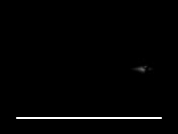
\includegraphics[width=\textwidth]{assets/5 results/ignitionFrames/16.jpg}
            \caption{\qty{1.6}{ms}}
            \label{fig:ignition_frames_16}
        \end{subfigure}
        \hfill
        \begin{subfigure}[t]{0.3\textwidth}
            \centering
            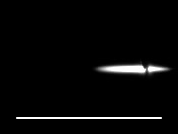
\includegraphics[width=\textwidth]{assets/5 results/ignitionFrames/17.jpg}
            \caption{\qty{1.7}{ms}}
            \label{fig:ignition_frames_17}
        \end{subfigure}
        \hfill
        \begin{subfigure}[t]{0.3\textwidth}
            \centering
            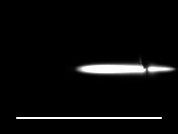
\includegraphics[width=\textwidth]{assets/5 results/ignitionFrames/18.jpg}
            \caption{\qty{1.8}{ms}}
            \label{fig:ignition_frames_18}
        \end{subfigure}
        \begin{subfigure}[t]{0.3\textwidth}
            \centering
            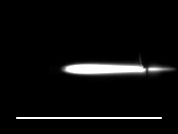
\includegraphics[width=\textwidth]{assets/5 results/ignitionFrames/19.jpg}
            \caption{\qty{1.9}{ms}}
            \label{fig:ignition_frames_19}
        \end{subfigure}
        \hfill
        \begin{subfigure}[t]{0.3\textwidth}
            \centering
            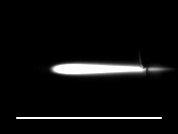
\includegraphics[width=\textwidth]{assets/5 results/ignitionFrames/20.jpg}
            \caption{\qty{2.0}{ms}}
            \label{fig:ignition_frames_20}
        \end{subfigure}
        \hfill
        \begin{subfigure}[t]{0.3\textwidth}
            \centering
            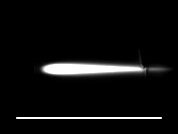
\includegraphics[width=\textwidth]{assets/5 results/ignitionFrames/21.jpg}
            \caption{\qty{2.1}{ms}}
            \label{fig:ignition_frames_21}
        \end{subfigure}
        \caption[LSP ignition via Tungsten wire]{LSP ignition via Tungsten wire: \qty{3080}{W}, \qty{20.29}{bar}. The white line at the bottom of each frame is \qty{10}{mm} long. \shotsettings{LSP1\_PS1}{0.1}{22}{2048}}
        \label{fig:ignition_frames}
    \end{figure}

    \begin{figure}[h]
        \centering
        \begin{subfigure}[t]{0.47\textwidth}
            \centering
            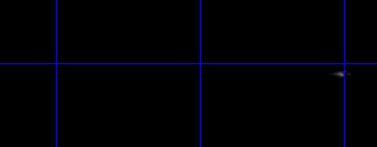
\includegraphics[width=\textwidth]{assets/5 results/1msFrames/16.jpg}
            \caption{\qty{1.6}{ms}}
            \label{fig:growth_frames_16}
        \end{subfigure}
        \hfill
        \begin{subfigure}[t]{0.47\textwidth}
            \centering
            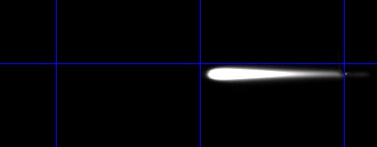
\includegraphics[width=\textwidth]{assets/5 results/1msFrames/26.jpg}
            \caption{\qty{2.6}{ms}}
            \label{fig:growth_frames_26}
        \end{subfigure}
        \hfill
        \begin{subfigure}[t]{0.47\textwidth}
            \centering
            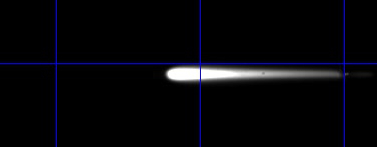
\includegraphics[width=\textwidth]{assets/5 results/1msFrames/36.jpg}
            \caption{\qty{3.6}{ms}}
            \label{fig:growth_frames_36}
        \end{subfigure}
        \hfill
        \begin{subfigure}[t]{0.47\textwidth}
            \centering
            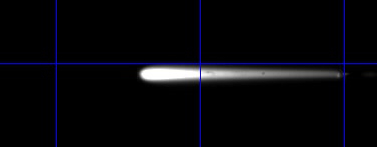
\includegraphics[width=\textwidth]{assets/5 results/1msFrames/46.jpg}
            \caption{\qty{4.6}{ms}}
            \label{fig:growth_frames_46}
        \end{subfigure}
        \hfill
        \begin{subfigure}[t]{0.47\textwidth}
            \centering
            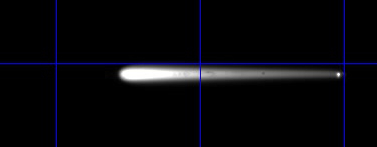
\includegraphics[width=\textwidth]{assets/5 results/1msFrames/56.jpg}
            \caption{\qty{5.6}{ms}}
            \label{fig:growth_frames_56}
        \end{subfigure}
        \hfill
        \begin{subfigure}[t]{0.47\textwidth}
            \centering
            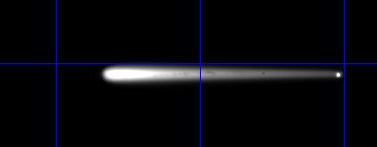
\includegraphics[width=\textwidth]{assets/5 results/1msFrames/66.jpg}
            \caption{\qty{6.6}{ms}}
            \label{fig:growth_frames_66}
        \end{subfigure}
        \hfill
        \begin{subfigure}[t]{0.47\textwidth}
            \centering
            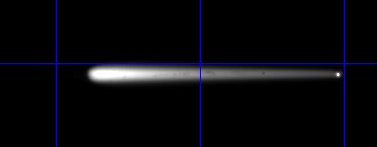
\includegraphics[width=\textwidth]{assets/5 results/1msFrames/76.jpg}
            \caption{\qty{7.6}{ms}}
            \label{fig:growth_frames_76}
        \end{subfigure}
        \hfill
        \begin{subfigure}[t]{0.47\textwidth}
            \centering
            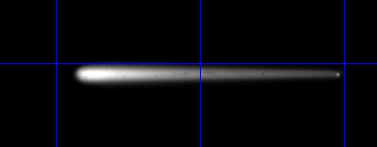
\includegraphics[width=\textwidth]{assets/5 results/1msFrames/86.jpg}
            \caption{\qty{8.6}{ms}}
            \label{fig:growth_frames_86}
        \end{subfigure}
        \hfill
        \begin{subfigure}[t]{0.47\textwidth}
            \centering
            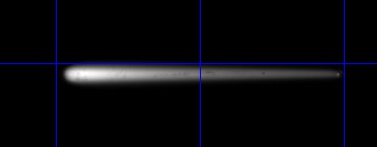
\includegraphics[width=\textwidth]{assets/5 results/1msFrames/96.jpg}
            \caption{\qty{9.6}{ms}}
            \label{fig:growth_frames_96}
        \end{subfigure}
        \hfill
        \begin{subfigure}[t]{0.47\textwidth}
            \centering
            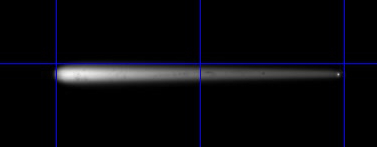
\includegraphics[width=\textwidth]{assets/5 results/1msFrames/106.jpg}
            \caption{\qty{10.6}{ms}}
            \label{fig:growth_frames_106}
        \end{subfigure}
        \hfill
        \begin{subfigure}[t]{0.47\textwidth}
            \centering
            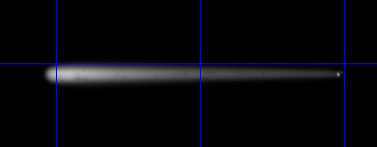
\includegraphics[width=\textwidth]{assets/5 results/1msFrames/116.jpg}
            \caption{\qty{11.6}{ms}}
            \label{fig:growth_frames_116}
        \end{subfigure}
        \caption[LSP growth throughout \qty{10}{ms} laser pulse]{LSP growth throughout \qty{10}{ms} laser pulse: \qty{3080}{W}, \qty{20.29}{bar}. The blue grid is spaced by \qty{10}{mm}. \shotsettings{LSP1\_PS1}{0.1}{22}{2048}}
        \label{fig:growth_frames}
    \end{figure}

    \begin{figure}[h]
        \centering
        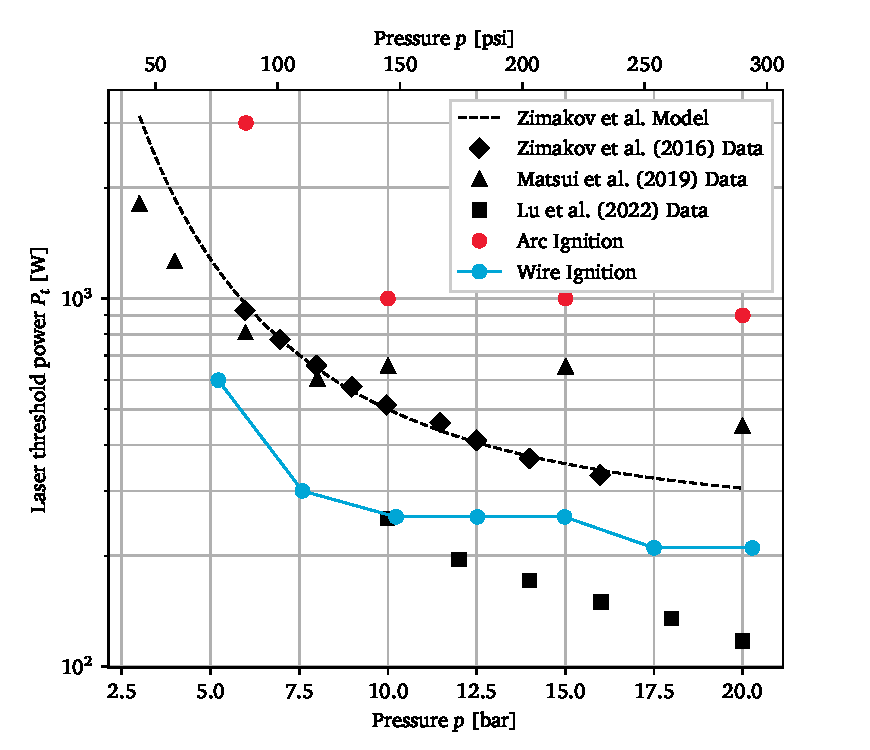
\includegraphics[]{assets/5 results/powerthreshold.pdf}
        \caption[Pressure-Power LSP threshold exploration]{Pressure-Power LSP threshold exploration. Experimental data for two different ignition methods is compared to past literature.}
        \label{fig:powerthreshold}
    \end{figure}